\documentclass[a4paper,12pt]{article}
\usepackage[a4paper, margin=1in]{geometry}
\usepackage[utf8]{inputenc}
\usepackage{graphicx}
\usepackage{xcolor}
\usepackage{braket}
\usepackage{amsmath} 
\usepackage{amssymb}
\usepackage[headings]{fancyhdr}
\graphicspath{ {./Figures/} }
\usepackage[sorting=none]{biblatex}
\addbibresource{refs.bib}

\usepackage{hyperref}
\hypersetup{
    colorlinks=true,
    linkcolor=black,
    urlcolor=cyan,
    citecolor=blue
}

\newcommand{\mytodo}[1]{\textcolor{red}{TODO: #1}}
\newcommand{\thetas}{\vec{\theta}}
\newcommand{\del}{\partial}
\newcommand{\base}{\mathcal{B}}
% \newcommand{\tvect}[2]{%
%   \ensuremath{\Bigl(\negthinspace\begin{smallmatrix}#1\\#2\end{smallmatrix}\Bigr)}}

\newcommand{\tvect}[2]{{#1 \choose #2}}

\DeclareMathOperator{\tr}{Tr}
\DeclareMathOperator{\Var}{Var}

\newtheorem{definition}{Definition}
\newtheorem{theorem}{Theorem}



\title{Mutual Unbiased Bases as a Countermeasure to Barren Plateaus in Variational Quantum Algorithms}

\author{Ittay Alfassi\footnote{Email: ittay.al@cs.technion.ac.il}}

\begin{document}
\maketitle

\thispagestyle{fancy}
\fancyhead[RO]{Project Supervisor:\\{Prof. Tal Mor}}
\fancyhead[LO]{{Project in Advanced Programming - 236503}\\{Project Report}}

\tableofcontents

\section{Introduction}
Noisy, Intermediate-Scale Quantum (NISQ) computers are quantum computers that are limited in certain ways. They are usually limited in the number of qubits, connectivity between qubits, noise, and maximal circuit depth.
A computational paradigm that utilizes NISQ devices is the paradigm of hybrid quantum-classical algorithms.
Most hybrid algorithms translate a given problem into an optimization problem.
The parameters of the optimization problem control some parametrized quantum state, the problem's cost function is evaluated on the quantum computer, and the optimization steps are performed by the classical computer. These algorithms are called Variational Quantum Algorithms (VQAs)~\cite{Cerezo2021}. \mytodo{Make sure this is accurate!}

While being a leading methodology for the use of quantum computers today, VQAs suffer from several problems. One such problem is the problem of Barren Plateaus~\cite{mcclean_barren_2018}. Informally, barren plateaus imply that over the optimization parameter space, the gradient of the cost function is negligibly small and the optimization process does not how to converge.

This problem affects many  VQAs that employ different types of quantum circuits and classical optimizers (even those that are gradient-free). As the number of qubits and the depth of the quantum circuits increase, this problem worsens exponentially.
Effectively, this means that VQAs will not be able to give an advantage over their classical counterparts in problems that are not small in size.

To address this issue, in this project, I will try and utilize Mutually Unbiased Bases (MUBs), their states, and their properties.
The basic intuition behind this method is that, for any number of qubits, the set of all MUB states spans the entire Hilbert space (with real coefficients).

Thus, inserting them (in some fashion) into the optimization process can allow for an ``exhaustive search'' over the Hilbert space of all states.

Unfortunately, this method did not succeed. However, I will detail the different aspects of this approach, the experiments implemented, the conclusions I reached, and possible methods to still utilize the idea of MUB states in VQAs.

This project is mainly based on the work of Arrasmith et al.~\cite{arrasmith_effect_2021}.


\section{Preliminaries}

\subsection{Variational Quantum Algorithms}
A Variational Quantum Algorithm is an algorithm that takes some computational problem and solves it by hybrid classical-quantum optimization.
VQAs are comprised of several elements: The quantum circuit, the cost function, and the optimizer.

\begin{enumerate}
    \item \textbf{The Quantum Circuit.} Every VQA problem uses a quantum circuit with some parametric values.
    Its structure can be generally written as the following:
    \begin{equation}
        U(\thetas) = \prod_{l=1}^{L} U_l(\theta_l) W_l
    \end{equation}
    Where $U_l(\theta_l) = \exp(-i\theta_l V_l)$, $V_l$ is a Hermitian operator (thus $U_l$ is a unitary operator), and $W_l$ is a generic unitary operator that does not depend on any angle $\theta_l$.
    
    In some VQAs, an \textbf{initial state} $\ket{\psi_0}$ is also a part of the algorithm, and it is related to the quantum circuit.

    The term \emph{ansatz} (German for ``approach''/``attempt'') is used in literature to either describe the initial state $\ket{\psi_0}$, the parametric circuit $U(\thetas)$, or the application of the parametric circuit to the initial state $\ket{\psi(\thetas)} = U(\thetas)\ket{\psi_0}$.
    In this project, I will use the term ansatz to refer to the parametric quantum circuit.

    Ansatzes\footnote{The plural form of ansatz in German is Ansaetze.} can either be problem-specific or problem-agnostic.

    A problem-specific ansatz is tailored to the problem solved by the VQE using a-priori knowledge of the structure of the problem. Through this tailoring, there is a better chance that the circuit can reach values that are optimal for the problem at hand. When using a problem-specific ansatz, the initial state is usually also tailored according to the same information.
    
    A problem-agnostic ansatz is not tailored to the problem specifically and can be used with no relevant information. It is usually comprised of repeated layers of quantum gates. Each layer is comprised of quantum gates that are usually easy to implement directly on quantum hardware, in contrast to problem-specific ansatzes. Problem-agnostic ansatzes are usually called ``hardware-efficient'' for this reason.
    In this project, I focused on using hardware-efficient ansatzes.
    
    \item \textbf{The Cost Function.} The cost function $C(\thetas)$ defines the goal of the VQA. It is defined as a function from the parameters of the ansatz to the real numbers.
    The goal of the VQA is to find
    \begin{equation}
        \thetas^* = \arg\min_{\thetas} C(\thetas)
    \end{equation}

    The cost function always depends on the ansatz, some Hermitian operators, and some initial states.
    Generally, it can be written as
    \begin{equation} \label{eqn:general_cost}
        C(\thetas) = \sum_k f_k(\tr[O_k U(\thetas) \rho_k U^\dagger(\thetas)])
    \end{equation} 
    Where $\{f_k\}$ is a set of functions, $\{O_k\}$ is a set of operators, and $\{\rho_k\}$ is a set of input states.
    
    The trademark of VQAs is that they use a quantum computer to estimate the cost function $C(\thetas)$ (or its derivatives) while leveraging the power of classical optimizers to train the parameters $\thetas$.
    
    \item \textbf{The Optimizer.} While not necessarily dependent on the problem the VQA is trying to solve, the classical optimizer is an important part of the algorithm.
    The optimizer is run on a classical computer, and performs an iterative process: it uses data on the current parameters of the cost function to calculate their value in the next iteration. More details can be found in subsection~\ref{subsec:optimizers}.
\end{enumerate}


\subsubsection{Example: Variational Quantum Eigensolver} \label{subsec:vqe}
One of the earliest examples of a VQA is the VQE algorithm, proposed by Peruzzo et al.~\cite{peruzzo_variational_2014}. In this algorithm, The goal is to find the lowest eigenvalue of some Hamiltonian $H$.
The cost function is straightforwardly defined as the expectation value of the parametric state over the Hamiltonian:

\begin{equation} \label{eqn:vqe_cost}
    C(\thetas) = \bra{\psi(\thetas)} H \ket{\psi(\thetas)} = \bra{\psi_0} U^\dagger(\thetas) H U(\thetas) \ket{\psi_0}
\end{equation}

In case $H$ is a molecular Hamiltonian (converted to a qubit Hamiltonian using an appropriate transformation), a problem-specific ansatz can be used. One such option is the Unitary Coupled-Cluster (UCC) ansatz, together with the Hartree-Fock state as the initial state.

Of course, a hardware-efficient ansatz can be used for any structure of $H$.

\subsubsection{Example: Variational Quantum Compiling} \label{subsec:vqc}
A different example of a VQA is the problem of Variational Quantum Compiling (VQC), initially defined by Khatri et al.~\cite{khatri_quantum-assisted_2019} as Quantum-Assisted Quantum Compiling (QAQC).

In VQC, the input of the problem is a general $n$-qubit unitary operation $V$.\footnote{In the Khatri paper, the target unitary is denoted as $U$, while the ansatz is denoted $V$. I switched the notations to stay consistent with the rest of the examples and papers.} The goal of the algorithm is to control the parameters of a parametric quantum circuit $U(\thetas)$ so its behavior will be similar to that of $V$.

Formally, there are two possible goals: either that $U(\thetas)$ and $V$ will perform the same operation on all states, or that $U(\thetas)$ and $V$ will perform the same operation on a specific input state.
In this project, I will use the latter as the problem definition. Thus, we wish that $V\ket{\vec{0}} = U(\thetas)\ket{\vec{0}}$.

There are two different cost functions presented in~\cite{khatri_quantum-assisted_2019}.
The first is straightforward and is defined by

\begin{equation}
    C^{\textrm{global}} = 1 - \left|\bra{\vec{0}}UV^\dagger\ket{\vec{0}}\right|^2
\end{equation}

Another cost function, called the local cost function, is defined by 

\begin{equation}
    C^{\textrm{local}} = 1 - \frac{1}{n} \sum_{j=1}^{n} p_0^{(j)}
\end{equation}

where
\begin{equation} \label{eqn:local_vqc_cost}
    p_0^{(j)} = \tr[({\ket{0}\bra{0}}_j \otimes I) U^\dagger V \ket{\vec{0}}\bra{\vec{0}} V^\dagger U]
\end{equation}
and ${\ket{0}\bra{0}}_j \otimes I$ is the tensor product of the matrix $\ket{0}\bra{0}$ in the jth term and identity matrices in all other terms.
The operational meaning of $p_0^{(j)}$ is the probability to obtain the zero measurement outcome on qubit $j$ for the state $U^\dagger V\ket{\vec{0}}$.

it is proven in~\cite{sharma_noise_2020} that

\begin{equation}
    C^{\textrm{local}} \leq C^{\textrm{global}} \leq nC^{\textrm{local}}
\end{equation} 

However, $C^\textrm{global}$ suffers from a provably vanishing gradient as $n$ increases, while $C^\textrm{local}$ does not. Thus, we will use $C^\textrm{local}$ or a linear combination of both costs in our experiments.

\subsection{Optimizers for Variational Quantum Algorithms} \label{subsec:optimizers}
Classical optimizers perform the task of finding a (hopefully global) extremum of some scalar function.
An optimizer for a function $F$ needs to find the vector $\thetas \in S$ with $S \subseteq \mathbb{R}^n$ that gives a minimal or maximal value for $F$. In this project, we will only use optimizers for the minimization of cost functions.

In each step, an optimizer is given a point in the parameter space of the cost function $\thetas_{i}$, and is tasked with finding a new guess for parameter values $\thetas_{i+1}$, which hopefully has a lower cost value.

The optimizer can either use the value of the cost function, its partial derivative (its gradient vector), or its second partial derivatives (its Hessian matrix).

Methods that use the second derivative are often called Newton methods (as Newton's method uses the second derivative). Methods that use \emph{approximations} of the first and second derivative are called Quasi-Newton methods.
Methods that use the first derivative are called Gradient-Based methods. Methods that do not use the derivative at all are called Gradient-Free methods.

In this project, I focused on two gradient-free optimizers: the Powell optimizer and the COBYLA optimizer.

\subsubsection{Powell}
The Powell algorithm~\cite{Powell1964} is a popular gradient-free optimizer that uses sequential line searches (optimizations over lines in the parameter space).

This method starts with some input set of search vectors $V = \{\vec{v}_i\}$, which are usually chosen to be the coordinate vectors in the parameter space. Each vector defines a search direction (both the direction of the vector and its negation).

Searching along each of those directions in sequence, this method looks for the displacement $\{a_i\}$ along each direction that would minimize the cost when only varying parameters along the current direction.
If bounds to the parameter space are specified, the minimization will be under said bounds. If bounds are not provided, then an unbounded line search will be used.
Finding the displacements in each direction is done by some univariate gradient-free optimizer.
Two common options for such an optimizer are Brent's parabolic interpolation method and the Golden-section search method, but their choice is independent of the general Powell method.

After sweeping through all of the search vectors, two updates are made:
First, the current parameters are updated by the rule:
\begin{equation}
    \thetas_{i+1} = \thetas_{i} + \sum_i a_i \vec{v}_i
\end{equation}
Second, the search vector $\vec{v}_j$ that corresponds to the greatest displacement, $a_j = \max(a_i)$ is replaced with
\begin{equation}
    \vec{v_j} \to \sum_i a_i \vec{v}_i.
\end{equation}

The algorithm iterates an arbitrary number of times until no significant improvement to the value of the cost function is made.


\subsubsection{COBYLA}
Constrained Optimization BY Linear Approximation (COBYLA) is a gradient-free numerical optimization method, invented by Powell~\cite{Powell1994,powell_view_2007} (although it is different from the Powell optimization method).

The method tries to optimize a function $F(\thetas)$ according to a set of constraints $\{c_i(\thetas)\}$.

At each iteration, the method has $m+1$ points $\{\thetas_i\}_{i=0}^m$ in the parameter space that are sorted by a combination of the function's value on them and the penalties that the constraints imply on them.
The said sorting function is of the form
\begin{equation}
    \Phi(\thetas) = F(\thetas) + \mu[ \max\{-c_i(\thetas) : i=1,2,\dots,m \} ]_+, \thetas \in \mathbb{R}^n
\end{equation}
For a value $\mu$ that is automatically controlled by the method and the subscript + signifying that 0 is taken in case the value of the expression is negative.
Thus, our points are sorted as $\Phi(\thetas_0) < \Phi(\thetas_1) < \dots < \Phi(\thetas_m)$.

In addition, there is a ``trust region'' with a radius $\rho>0$. The method uses the $m+1$ points as the vertices of a simplex (an $m$-dimensional generalization of a triangle).
The values of the cost function in these vertices are used for interpolation to a unique linear polynomial $\hat{F}(\thetas)$, and the values of the constraint functions in these vertices are used for interpolation to unique linear constraints $\{\hat{c}_i\}$
The method then continues by minimizing $\hat{F}(\thetas)$, which is in the trust region --- that is, $\frac{\rho}{2} \leq \|\thetas - \thetas_0\| \leq \rho$, under the approximated constraints $\{\hat{c}_i\}$.

In case there is no point in the trust region in which all approximated constraints are satisfied, $\thetas$ is defined by minimizing the greatest of the constraint violations subject to the trust region bound.

The newly calculated point is added to the set of points, and some other point is removed.
The choice of the point to be removed is governed mainly by avoiding the degenerate situation where the volume of the simplex collapses to zero, as in that case, only a subspace of the parameter space is reachable.

When the improvements are insufficient, the value of $\rho$ is reduced, until some lower bound, which specifies the termination of the method, is reached.

This explanation of the method is incomplete, and only describes the general principle behind the optimization. In addition, different specifications by Powell (for example, \cite{Powell1994} and \cite{powell_view_2007}) define certain requirements and symbols differently, such as using $\Phi$ or $F$ for the sorting of vertices, the use of $\mu$, and the use of $\rho$ as the trust radius or as a lower bound for it.
Certain technical details and special steps in the method are also omitted and can be found in section 2 of~\cite{Powell1994}.


\section{Barren Plateaus} \label{sec:bps}
Informally, a barren plateau is a large section of the parameter space in which the value of the cost function $C$ is ``flat'', and has no apparent direction in which to move in order to reach a minimum point. The term was first coined by McClean et al. in~\cite{mcclean_barren_2018}.

When considering a cost function with 2 parameters, this definition coincides with its geometrical intuition. The plane defined by $\{(\theta_1, \theta_2, C(\theta_1, \theta_2)) | (\theta_1, \theta_2) \in \mathbb{R}^2\}$ will have large, flat sections, in which the ``dips'' that represent minima are not indicated by a slope around them (other than a very small neighborhood of the minimum). Such an example can be seen in Figure~\ref{fig:bp}.

\begin{figure}[h]
    \centering
    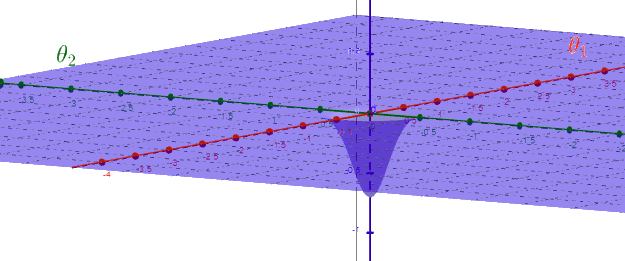
\includegraphics[scale=0.5]{bp_3d.png}
    \caption{A barren plateau in an inverted bi-variate Gaussian with a small variance.}
    \label{fig:bp}
\end{figure}

This is formally defined by the expectation value and variance of the partial derivatives.
As defined in \cite{arrasmith_effect_2021}:

\begin{definition} \label{def:bp}
    Consider the cost function defined in Eq.~(\ref{eqn:general_cost}). This cost exhibits a barren plateau if, for all $\theta_\mu \in \thetas$, the expectation value of the cost function partial derivative
    $\del C / \del\theta_\mu = \del_\mu C(\thetas)$
    is
    $E_{\thetas}[\del_\mu C(\thetas)] = 0$
    and its variance vanishes exponentially with the number of qubits n as 
    \begin{equation} \label{eqn:vanishing}
        \Var_{\thetas}[\del_\mu C(\thetas)] \leq F(n) \textrm{,   with   }F(n) \in O\left(\frac{1}{b^n}\right)
    \end{equation}
    for some $b > 1$. As indicated, the expectation values are taken over the parameters $\thetas$.
\end{definition}

\subsection{Ansatzes and Functions Affected By Barren Plateaus}
Papers in the field of barren plateaus have shown that many types of cost functions exhibit barren plateaus.

The original work by McClean et al.~\cite{mcclean_barren_2018} shows that cost functions of the form in Eq. (\ref{eqn:general_cost}) that use random quantum circuits of polynomial depth and exhibit a property known as a \emph{2-design} suffer from barren plateaus.
The definition of a 2-design is beyond the mathematical scope of this project.

However, the work of Arrasmith et al.~\cite{arrasmith_effect_2021} notes that hardware-efficient layered ansatzes are approximate 2-designs (although they did not show this result themselves).
As such, cost functions that use these ansatzes suffer from barren plateaus when the number of layers scales linearly with the number of qubits.

Another paper, by Cerezo et al.~\cite{cerezo_cost_2021}, shows that if the cost function makes use of global operators, barren plateaus will be encountered in \emph{any} circuit depth.
For this reason, it is preferable to use the local cost function in VQC problems and not the global cost function.
% A paper by Wang et al.~\cite{wang_noise-induced_2021}

\subsubsection{Barren Plateaus in VQC}
In section 4 of Arrasmith~\cite{arrasmith_effect_2021}, it is shown that even a fairly simple VQC problem suffers from barren plateaus.

The specific problem shown in the paper is concerned with the trivial target unitary $V = I$.
Thus, we are trying to optimize the parameters of a parametric quantum circuit $U(\thetas)$ such that $U(\thetas)\ket{\vec{0}} = I\ket{\vec{0}} = \ket{\vec{0}}$.

The quantum circuit used is a layered hardware-efficient ansatz.
Each layer is defined by the following structure:
\begin{itemize}
    \item A general unitary single-qubit rotation gate $U(\theta_1, \theta_2, \theta_3)$ gate is applied to each qubit.
    \item A layer of Control-NOT gates is applied between even pairs of qubits (that is, even indices act as controls and odd indices act as targets).
    \item Another layer of general unitary single-qubit rotations is applied.
    \item A layer of Control-NOT gates is applied between odd pairs of qubits (odd indices act as controls and even indices act as targets).
\end{itemize}
A sketch of a single layer of the circuit can be seen in Figure~\ref{fig:layer}.

The cost function used is the local VQC cost function, as shown in Eq. (\ref{eqn:local_vqc_cost}).
Arrasmith~\cite{arrasmith_effect_2021} claims that when the number of layers scales linearly with the number of qubits, this problem instance suffers from barren plateaus.

\begin{figure}[h]
    \centering
    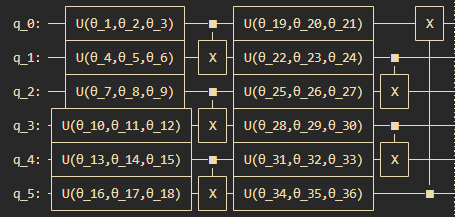
\includegraphics{arrasmith_layer.png}
    \caption{A single layer of the hardware-efficient ansatz used in the project, as designed in Qiskit.}
    \label{fig:layer}
\end{figure}

\subsection{Barren Plateaus in Gradient-Free Optimization}
Seeing as the definition of barren plateaus only discusses the partial derivatives of the cost function, one might assume that using gradient-free optimizers solves this issue.
However, the main result of Arrasmith shows that this is incorrect.

The following theorem is shown in~\cite{arrasmith_effect_2021}:

\begin{theorem}
    Consider the cost function of Eq.~(\ref{eqn:general_cost}). Let ${\thetas}_A$ and $\thetas_B$ be two randomly chosen points in parameter space.
    Without loss of generality we assume that $\thetas_B = \thetas_A + L\hat{l}$ for random $L$ and $\hat{l}$ so that $E_{\thetas_A, \thetas_B}[\dots] = E_{\thetas_A, L, \hat{l}}[\dots]$.
    If the cost exhibits a barren plateau according to Definition~\ref{def:bp}, then the expectation value of the difference $\Delta C = C(\thetas_B) - C(\thetas_A)$ is $E_{\thetas_A, L, \hat{l}}[\Delta C] = 0$, and the variance is exponentially vanishing with n as 
    \begin{equation}
        \Var_{\thetas_A,L,\hat{l}}[\Delta C] \leq \hat{G}(n)
    \end{equation}
    with
    \begin{equation}
        \hat{G}(n) = m^2 \bar{L}^2 F(n)\textrm{,    and     } \hat{G}(n) \in \tilde{O}\left(\frac{1}{b^n}\right).
    \end{equation}
    for some $b>1$. Here m is the dimension of the parameter space, $F(n)$ was defined in (\ref{eqn:vanishing}), and
    \begin{equation}
        \bar{L} = E_{L,\hat(l)}[L]
    \end{equation}
    is the average distance between any two points in parameter space.
\end{theorem}

The effective meaning of this theorem is that the difference in the cost function between different points in the parameter space is exponentially vanishing in $n$.
Thus, even though gradient-free optimizers do not use derivatives, they are still affected --- Their main tool for decision-making, which is the difference in the values of the function, gives almost no information.

\section{Mutually Unbiased Bases}
The state space of an $n$-qubit system is a $2^n$ dimensional Hilbert space.
As such, an orthonormal basis for said space contains $2^n$ distinct vectors.
There are infinitely many bases for such a space, but some combinations of bases exhibit special properties. One property, which is the main focus of this project, is \emph{Mutual Unbias}.

The following is a definition for Mutually Unbiased Bases~\cite{bandyopadhyay_new_2002}:
\begin{definition}
    Let $\base_1 = \{\ket{\phi_i}\}$ and $\base_2 = \{\ket{\psi_i}\}$ be two orthonormal bases in the $d$ dimensional state space.
    They are said to be \textbf{mutually unbiased bases (MUB)} iff the following holds:
    \begin{equation}
        \forall i,j : |\langle \psi_i | \phi_j \rangle | = \frac{1}{\sqrt{d}}
    \end{equation}
    A set $\{\base_1,\dots,\base_m\}$ of orthonormal bases in $\mathbb{C}^d$ is called a \emph{set of mutually unbiased bases} (a set of MUB) if each pair of bases $\base_i$ and $\base_j$ are mutually unbiased.
\end{definition}

The intuition for such a definition is that, if a state from one basis is measured in the other, every measurement possibility has equal probability.

In general, the term ``MUB set'' refers to a set of bases that are pairwise mutually unbiased.
The term ``MUB states'', in the context of some MUB set, is the collection of states that comprises the MUBs of that set.

\subsection{Generation of Mutually Unbiased Bases} \label{subsec:mub_gen}
The question of the existence, number, and generation of MUB sets is only answered for certain cases.

The following result has been achieved~\cite{bandyopadhyay_new_2002}:
For an $d$-dimensional state space, if $d$ is prime or a prime power ($p^k$ for a prime $p$ and a natural number $k$), there exists a set of $d+1$ MUBs.
There is constructive proof for this result.
Because the dimension of an $n$-qubit state space is $2^n$ (a prime power), there is a construction for $2^n+1$ MUBs for every $n$.

It is important to note, of course, that once a MUB set is found, there is an infinite amount of possibilities for MUB sets of the same size. Applying any arbitrary unitary $U$ to all states of the set of bases will preserve the constraints on the inner products of every pair of states, which gives a new MUB set (assuming $U$ did not act as a permutation on the set).

Connections between the problem of finding MUB sets and other problems have been made. For example, Lawrence et al.~\cite{lawrence_mutually_2002} showed that the set of $4^n-1$ Pauli operators (in the $n$-qubit case) can be partitioned into $2^n+1$ distinct subsets, each consisting of $2^n-1$ commuting operators. The same work shows two interesting conclusions:
\begin{itemize}
    \item The set of eigenbases that mutually diagonalize each subset is a set of MUBs.
    That is, if each subset $\mathcal{F}_i$ is mutually diagonalized by an orthonormal basis $\base_i$, then the set $\{\base_i\}$ is a MUB set.
    \item Each such partitioning defined a unique choice of $2^n+1$ MUBs in the $n$-qubit Hilbert space.
\end{itemize}

I used the examples given in the work of Lawrence et al. to construct a set of MUBs for 2 and 3 qubits.
However, it is important to note that the generation of MUBs in this fashion requires exponential time in the number of qubits: it requires the simultaneous diagonalization of matrices that are exponential in size.

\subsection{MUB States as an Exhaustive Search}

The set of MUB states for 1 qubit is well known. The set contains 3 MUBs, and each basis is the eigenbasis of a Pauli matrix.
Specifically, the bases and states are
$$ \base_z = \{ \ket{0}, \ket{1}\}  = \{\tvect{1}{0}, \tvect{0}{1}\}$$
$$ \base_x = \{ \ket{+}, \ket{-}\}  = \{\frac{1}{\sqrt{2}}\tvect{1}{1}, \frac{1}{\sqrt{2}}\tvect{1}{-1}\}$$
$$ \base_y = \{ \ket{+_i}, \ket{-_i}\}  = \{\frac{1}{\sqrt{2}}\tvect{1}{i}, \frac{1}{\sqrt{2}}\tvect{1}{-i}\}$$

When displayed on the Bloch sphere, these states are presented as the poles of the sphere in the z, x, and y axes, appropriately. As such, every 1-qubit state is reachable through a linear combination of these six states with real coefficients.

This is our initial intuition: these states reach every pole of the sphere that defines all 1-qubit states.
We (Tal Mor and I) believed that this can be extended to higher dimensions. If our hypothesis of the importance of MUBs is correct, they can be useful when trying to check for a certain property, \textbf{or when searching for a specific point in space.}

An observation made in~\cite{lawrence_mutually_2002} supports our hypothesis.
In~\cite{lawrence_mutually_2002}, a MUB is generated by being the orthonormal basis that mutually diagonalizes a subset of Pauli operators.
Let $\{O_i\}$ be such a subset of Pauli operators, and let $\{\ket{\psi_i}\}$ be the mutually diagonalizing eigenbasis calculated for that subset.
Let $U_i(\theta) = exp(-i\theta O_i)$ be a unitary high-dimensional rotation defined by $O_i$.
When $U_i$ acts on a MUB state $\ket{\psi_j}$, that state will not be affected (up to a global phase) \textbf{and act as a pole}.

In the next section, I will discuss the different methods to use the concept of MUB states as an exhaustive search in mitigating barren plateaus.


\section{MUB Utilization Techniques}
This section specifies the novel ideas that Tal and I had for the project. As such, they are comprised of theoretic extensions and assumptions that we made.

To explain our idea, let us consider a VQA in which the target is to reach a specific state.
One such example is VQE (section~\ref{subsec:vqe}), in which the lowest eigenvalue is calculated by reaching the lowest eigenstate.
An example of utilizing MUBs in a different type of VQA is given in subsection~\ref{subsec:mub_vqc}.

Let us make the following assumptions:
\begin{enumerate}
    \item The cost function $C(\thetas)$ (shown in Eq.~(\ref{eqn:vqe_cost})) experiences a barren plateau in the parameter space. 
    \item The optimization starts with a specific initial parameter vector, $\thetas_0$, whose entries were chosen uniformly randomly from the parameter space.
    \item The ansatz $U(\theta)$ is \emph{expressive} --- Every state $\ket{\psi}$ in the state has a parameter vector $\thetas_\psi$ such that $U(\thetas_\psi)\ket{\vec{0}} = \ket{\psi}$.
    \label{itm:expressive}
\end{enumerate}

The target state $\ket{\psi^*}$ that the VQA is trying to reach, according to assumption~\ref{itm:expressive}, has an appropriate parameter choice $\thetas^*$.
However, since $C(\thetas)$ suffers from barren plateaus, any optimizer cannot travel long distances in the parameter space.
Thus, if $U(\thetas_0)\ket{\vec{0}}$ is far from $\ket{\psi^*}$ (in terms of the state space), the VQA will not reach the required parameters.

However, because the MUB states act as an exhaustive search over the Hilbert space (or so we hope), there exists some MUB state $\ket{\alpha}$ such that $U(\thetas_0)\ket{\alpha}$ and $\ket{\psi^*}$ are close (in terms of the state space).
Equivalently, there exists some parameter vector $\thetas_0^\alpha$ such that $U(\thetas_0) \ket{\alpha} = U(\thetas_0^\alpha) \ket{\vec{0}}$, and $\thetas_0^\alpha$ and $\thetas^*$ are close \textbf{in terms of the parameter space}. Thus, an optimizer will be able to find an appropriate parameter set and reach $\ket{\psi^*}$ despite the barren plateaus of the cost function.

\paragraph*{Non-Uniformity of Parameter Space}~\\
An ansatz, even if fully expressive, does not necessarily bring its input to all output states in the Hilbert space with equal probability. For example, it could be that the vast majority of parameter vectors bring the result to a very small distance from the input vector.
For this reason, the use of a MUB state to dramatically shift the output result is valuable.
This phenomenon is connected to the mathematical term called \emph{Concentration of Measure} and to the Haar Measure for unitaries and states, as mentioned in~\cite{mcclean_barren_2018}.
However, the research of these terms and phenomena were left outside the scope of this report.

\paragraph*{Non-Expressive Ansatzes}~\\
While assumption~\ref{itm:expressive} seems useful (both for applications and for our analysis), it is unfortunately unrealistic.
Seeing as a general $2^n \times 2^n$ unitary matrix has an exponential number of degrees of freedom, reaching the entire set of unitary transformations requires an exponential number of parameters and an ansatz of exponential size.

Thus, the output of a hardware-efficient ansatz of linear depth will only span a small subset of the Hilbert space.
If our target is a state $\ket{\psi^*}$, it could lie outside the subset $\{U(\thetas)\ket{\vec{0}} | \thetas \in \mathbb{R}^m\}$. Using a MUB state as the input instead of $\ket{\vec{0}}$ could dramatically shift the subset and change it to include $\ket{\psi^*}$.

\medskip
The question that remains is how \emph{exactly} to use the set of MUB states.

\subsection{Using All MUB states}
The most trivial idea is to attempt optimization from all possible MUB states.
That is, set a specific random initial parameter vector $\thetas_0$, and run a separate experiment with every MUB state as the initial state.

However, there is a major drawback to this method.
For $n$ qubits, there are $2^n+1$ different MUBs, with $2^n$ states each.
Thus, this requires performing $O(4^n)$ experiments for every instance of the problem, which is non-scalable for reasonable problem sizes.

\subsection{Sampling $k$ MUB states}
A way to mitigate the drawback I just mentioned is to randomly sample a small number of MUB states from the entire set, and only run experiments from them.

This will allow an arbitrary amount of experiments, which we can control.
In addition, as will be discussed in section~\ref{subsec:random_thetas}, this serves as an interesting benchmark to compare against na{\"i}ve methods.

However, as mentioned in subsection~\ref{subsec:mub_gen}, the cost of calculation of the MUBs and their states is still exponential in time. Although the work of MUB calculation only needs to happen once and can be considered pre-processing, this makes the current suggestion unfeasible, for example, for $n>60$ qubits.

In addition, although the work of~\cite{bandyopadhyay_new_2002} shows a theoretical construction for the MUB sets for $n$ qubits, it is difficult to implement in practice.
Thus, Tal and I faced an interesting question: what can be done, for $n$ qubits, with only the MUB states for 2 and 3 qubits?

\subsection{``Half-MUB'' states}
We came up with a relatively simple idea: given an $n$-qubit register, pick 2 or 3 qubits. Generate a MUB state between the chosen qubits, and keep the rest in the 0 state.

The amount of such states for $n$ qubits is polynomial. There are ${n \choose 3} = O(n^3)$ triplets for the qubit choices, and each one has a constant amount of MUB state options.
Thus, their generation (and even exhaustive experimentation with them) takes reasonable time.

This method got the nickname ``Half-MUBs'', as its results resemble MUB states but do not give the same exhaustive properties.
However, no one guaranteed that MUB states act as an exhaustive search themselves, so what the hell.

\subsection{MUB Utilization in VQC} \label{subsec:mub_vqc}
As explained in subsection~\ref{subsec:vqc}, the goal of VQC is to make the ansatz act like a specific target unitary (either in general or on a specific state).
In this sense, it deviates from the previous discussions in this section, as it does not aim to reach a specific state, but a specific transformation.
However, the claims presented in this section still apply in the case of VQC.

The only difference is that instead of considering the state Hilbert space, we look at the group of unitary transformations on $n$ qubits $U(2^n)$.
Non-Uniformity still applies: a uniform choice of parameter values for the ansatz does not necessarily send the resulting unitary to a uniformly random unitary in $U(2^n)$.
Because of that, the prepending of the MUB generation circuit to the ansatz could move it dramatically closer to the target unitary (in terms of the parameter space).
Non-expressivity applies in a similar fashion.

\section{Experiments}

\subsection{Control Group: Random Initialization Vectors} \label{subsec:random_thetas}

\subsection{Experiment 1: Reproducing the Arrasmith Barren Plateau}

\subsection{Experiment 2: 3 qubits and $n$ layers}

\subsection{Experiment 3: $n$ qubits and $n$ layers}

\section{Discussion}

\section{Future Work}

\printbibliography
\end{document}
